\section{Results}
\label{sec:results}

\begin{figure}[t]
\centering
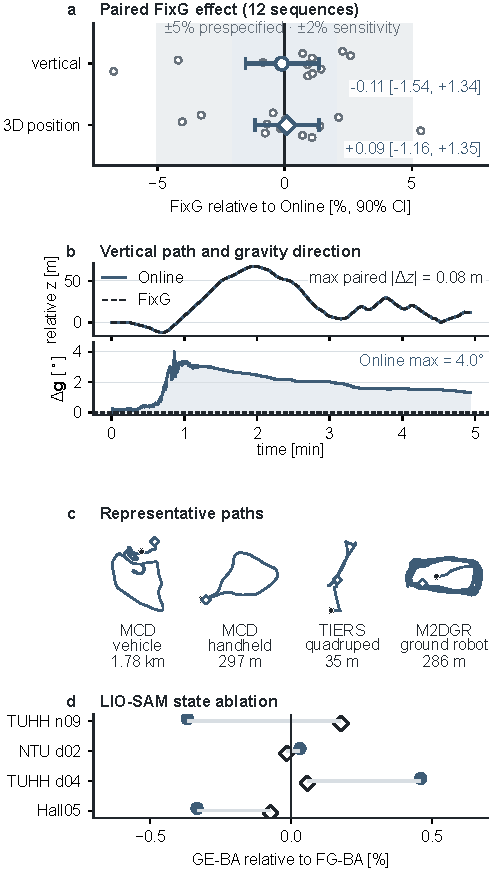
\includegraphics[width=\columnwidth]{figs/fig_factorial.pdf}
\caption{Continuous-correction state ablation. \textbf{a}, FAST-LIO2
mean paired effects with 90\% confidence intervals ($n=\NumCoreSeq{}$ paired
sequences; small symbols show individual effects). \textbf{b}, A paired
sequence in which online gravity moves while Online and FixG vertical estimates
remain nearly superposed; this trace is illustrative, not the population test.
\textbf{c}, Representative \methodA{} trajectories; XY scales are independent,
and path lengths come from admitted references.
\textbf{d}, Descriptive LIO-SAM transfer; circles denote RMSE$_z$ and
diamonds ATE (3D position error).}
\label{fig:factorial}
\end{figure}

\subsection{Structural Validation}
Structural logs verify the intended intervention before accuracy is examined.
Online gravity moves by as much as \GravWanderMax{}, while every removed
gravity trace is bit-exact and retains the prescribed magnitude. Online
$\mathbf b_a$ changes and fixed $\mathbf b_a$ does not. Paired correction
timestamps, admitted frame counts, and initial directions match. The early
fingerprint limitation is stated in Sec.~\ref{sec:method}. These logs confirm
distinct state treatments, not an accuracy benefit. The FAST-LIO2
nominal block contains \NumCoreRuns{} admitted trajectories across the four
configurations. In LIO-SAM, exact state dimensions match the intended structures,
and every admitted factor run contributes one direction factor at each audited
epoch. The final Hall05 reset is retained as a stability outcome without an
accuracy value; the earlier timestamp-misaligned run was excluded and rerun.

\subsection{Continuous-Correction State Ablation}
Across the \NumCoreSeq{} nominal sequences, the signed median RMSE$_z$ change
for \methodG{} is \GZMedian{}, and the median absolute change is
\GZAbsMedian{} (range \GZRange{}). The corresponding ATE values are
\GATEMedian{} and \GATEAbsMedian{} (range \GATERange{}). TOST places both
mean paired effects inside the pre-specified $\pm$\EquivMargin{} margin
(both $p$ values \EquivPBoth{}). Back-transformed mean effects and 90\%
intervals are \EquivCIZ{} for RMSE$_z$ and \EquivCIATE{} for ATE
(Fig.~\ref{fig:factorial}; Table~\ref{tab:nominal}). This supports average
practical equivalence, not a per-trajectory guarantee. Both metrics also pass
a post-hoc $\pm$\StrictEquivMargin{} sensitivity test (maximum $p$
\StrictEquivPBoth{}), while equal weighting across five trajectory families
retains the pre-specified decision (maximum $p$ \FamilyEquivPBoth{}). A
launch-fingerprint reproduction on the same sequence units gives
\ReproEquivCIZ{}/\ReproEquivCIATE{} and passes both margins (maximum strict
$p$ \ReproStrictEquivPBoth{}); it is a reproducibility check, not an
independent $n=24$ population.
The paired trace in Fig.~\ref{fig:factorial}b shows a moving gravity state
alongside nearly superposed vertical estimates. The equivalence result comes
from the paired population test, not this individual trace.

Absolute scale matters: median absolute \methodG{}--\methodA{} differences
are \FixGAbsDeltaZMedian{} for RMSE$_z$ and \FixGAbsDeltaATEMedian{} for ATE.
On m2dgr-hall, \HallFixGZ{} is only \HallFixGZDeltaMm{} in RMSE$_z$; its ATE
change is \HallFixGATE{} (\HallFixGATEDeltaMm{}). We therefore interpret paired
percentages with absolute differences and require both metrics, which can
disagree in sign.

The LIO-SAM state ablation yields a similar nominal pattern. Across
\NumLioSamSeq{} complete sequences, \lsGEBA{} relative to native \lsFGBA{}
changes RMSE$_z$ by \mbox{\LioSamGZRange{}} and ATE by
\mbox{\LioSamGATERange{}}; neither metric has a consistent sign. Fixing both
quantities changes RMSE$_z$/ATE by
\mbox{\LioSamBothZRange{}}/\mbox{\LioSamBothATERange{}}. These data provide a
descriptive cross-architecture check on the absent nominal gain from online
gravity. They do not establish LIO-SAM equivalence or a general rule for
$\mathbf b_a$.

\begin{table}[t]
\caption{State ablation with continuous correction.}
\label{tab:nominal}
\centering
\footnotesize
\setlength{\tabcolsep}{2.5pt}
% Auto-generated by scripts/make_tables.py; do not edit.
\begingroup
\renewcommand{\arraystretch}{1.06}
\newcommand{\nominalpair}[2]{\makebox[2.6em][r]{$#1$}\,$/$\,\makebox[2.6em][l]{$#2$}}
\begin{tabular*}{\columnwidth}{@{\extracolsep{\fill}}lcccc@{}}
\toprule
\rowcolor{TableBand}
\multicolumn{5}{@{}l}{\textsc{FAST-LIO2}\enspace paired change vs. \methodA{} [\%], $n=12$} \\
Configuration & dim. & median $z$/ATE & range $z$ & range ATE \\
\midrule
\methodG{} & 21 & \nominalpair{+0.9}{-0.1} & $[-6.7,+2.6]$ & $[-4.0,+5.4]$ \\
\methodB{} & 20 & \nominalpair{+1.5}{+0.2} & $[-2.1,+21.9]$ & $[-3.3,+12.6]$ \\
\methodGB{} & 18 & \nominalpair{+1.9}{+0.2} & $[-8.7,+47.2]$ & $[-6.1,+14.6]$ \\
\bottomrule
\end{tabular*}

\vspace{3pt}
\begin{tabular*}{\columnwidth}{@{\extracolsep{\fill}}lccc@{}}
\rowcolor{TableBand}
\multicolumn{4}{@{}l}{\textsc{LIO-SAM}\enspace paired $\Delta z/\Delta$ATE vs. \lsFGBA{} [\%]} \\
Sequence & \lsFGBZ{} & \lsGEBA{} & \lsGEBZ{} \\
\midrule
Hall05 & \nominalpair{+0.76}{+0.02} & \nominalpair{-0.33}{-0.07} & \nominalpair{+1.27}{+0.01} \\
TUHH d04 & \nominalpair{-3.20}{-1.09} & \nominalpair{+0.46}{+0.06} & \nominalpair{+0.93}{+0.16} \\
NTU d02 & \nominalpair{+0.04}{+0.02} & \nominalpair{+0.03}{-0.01} & \nominalpair{+0.00}{-0.04} \\
TUHH n09 & \nominalpair{-0.22}{+0.27} & \nominalpair{-0.37}{+0.18} & \nominalpair{-0.09}{+0.46} \\
\bottomrule
\end{tabular*}
\endgroup

\end{table}

\begin{figure}[t]
\centering
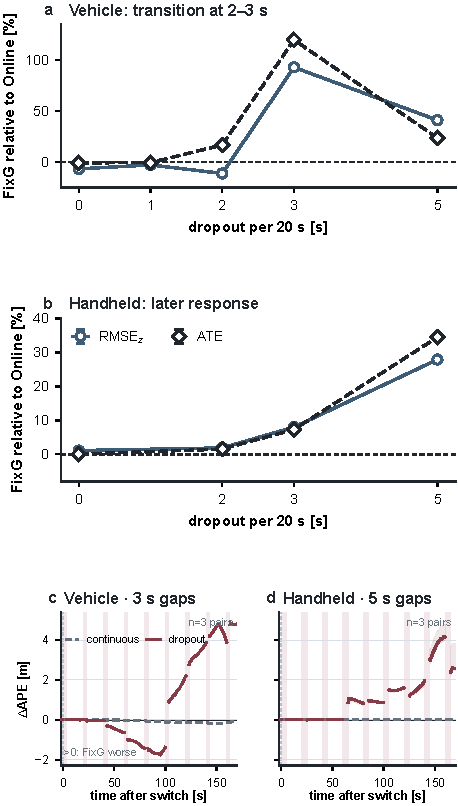
\includegraphics[width=\columnwidth]{figs/fig_boundary.pdf}
\caption{Correction-absence boundary. \textbf{a,b}, \methodG{} relative to
\methodA{} on vehicle and handheld trajectories; both RMSE$_z$ and ATE are
required. \textbf{c,d}, APE difference after the matched 23D-to-21D switch:
median and range across \NumWarmRepeatPairs{} serial pairs under a common
alignment. Shading denotes missing corrections; positive values favor Online.}
\label{fig:boundary}
\end{figure}

\subsection{Weak Geometry and Correction Absence}
Continuously degraded scans do not reproduce a dropout penalty. A 20\,m range
cap changes \methodG{} RMSE$_z$/ATE by \RangeGZ{}/\RangeGATE{}; a forward
$\pm60^\circ$ FoV changes them by \FovGZ{}/\FovGATE{}. Both retain scan-update
timing (Table~\ref{tab:operating}).

Complete dropout separates the designs. A 1-s gap every 20\,s remains benign.
At 2\,s, vehicle RMSE$_z$/ATE move in opposite directions
(\DropTwoGZ{}/\DropTwoGATE{}), so neither metric alone supports a configuration
choice. At 3\,s, both rise by \DropThreeGZ{}/\DropThreeGATE{} in all
\NumBoundaryRepeats{} serial repeats. The handheld response is later:
\HhsDropThreeGZ{}/\HhsDropThreeGATE{} at 3\,s and
\HhsDropFiveGZ{}/\HhsDropFiveGATE{} at 5\,s. Vehicle 5-s effects remain worse
than Online but are smaller than at 3\,s, so duration is not a monotonic dose.

The matched APE traces in Fig.~\ref{fig:boundary}c,d start at zero, stay near
zero with continuous correction, but separate progressively after repeated
gaps. The vehicle contrast initially changes sign; the handheld responds later.
The repeated trajectories do not show an effect confined to the first return.
The 2--3-s vehicle transition and later handheld response place the onset at
different gap durations, rather than a universal threshold.

The matched switch reproduces the regime contrast across
\NumWarmRepeatPairs{} serial pairs at the original dropout phase. Clean-input
ATE effects are small: \mbox{\WarmVehCleanATE{}} on the vehicle and
\mbox{\WarmHhsCleanATE{}} on the handheld trajectory. The median dropout-minus-clean
ATE interactions are \mbox{\WarmVehATEInteraction{}} and
\mbox{\WarmHhsATEInteraction{}}, respectively. Across \NumWarmPhases{}
dropout phases, ATE interactions are positive on both trajectories, whereas
RMSE$_z$ interactions cross zero (Table~\ref{tab:operating}). The stable effect
across these phases is therefore in 3D position error, not vertical error.

\begin{table}[t]
\caption{Correction-regime boundary.}
\label{tab:operating}
\centering
\footnotesize
\setlength{\tabcolsep}{2.8pt}
% Auto-generated by scripts/make_tables.py; do not edit.
\begin{tabular}{@{}lcccc@{}}
\toprule
Condition & \methodA{} $z$/ATE [m] & $\Delta z$ [\%] & $\Delta$ATE [\%] & $n$ \\
\midrule
\rowcolor{TableBand}
\multicolumn{5}{@{}l}{\textsc{Vehicle}\enspace continuous correction} \\
nominal & $2.49/6.60$ & $-6.7$ & $-0.8$ & 1 \\
range 20 m & $2.81/10.08$ & $+0.2$ & $-4.0$ & 1 \\
FoV $\pm60^\circ$ & $5.17/6.49$ & $+6.9$ & $+3.5$ & 1 \\
\addlinespace[2pt]
\rowcolor{TableBand}
\multicolumn{5}{@{}l}{\textsc{Vehicle}\enspace dropout per 20 s} \\
1 s/20 s & $2.43/6.50$ & $-2.8$ & $-0.5$ & 1 \\
2 s/20 s & $2.31/6.27$ & $-11.2$ & $+16.8$ & 3 \\
3 s/20 s & $3.09/8.42$ & $+93.1$ & $+119.9$ & 3 \\
5 s/20 s & $4.92/13.65$ & $+41.2$ & $+23.8$ & 1 \\
\addlinespace[2pt]
\rowcolor{TableBand}
\multicolumn{5}{@{}l}{\textsc{Handheld}\enspace dropout per 20 s} \\
2 s/20 s & $0.445/0.519$ & $+1.9$ & $+1.5$ & 1 \\
3 s/20 s & $0.485/0.536$ & $+8.0$ & $+7.3$ & 1 \\
5 s/20 s & $3.28/4.07$ & $+27.9$ & $+34.5$ & 1 \\
\addlinespace[2pt]
\rowcolor{TableBand}
\multicolumn{5}{@{}l}{\textsc{Matched posterior switch}\enspace dropout--clean interaction [m]} \\
vehicle repeats & -- & $+0.62$ & $+4.16$ & 3 \\
vehicle phases & -- & $[-0.23,+2.74]$ & $[+0.87,+4.16]$ & 3 \\
handheld repeats & -- & $+0.09$ & $+1.01$ & 3 \\
handheld phases & -- & $[-0.08,+0.22]$ & $[+0.30,+1.09]$ & 3 \\
\bottomrule
\end{tabular}

\end{table}

\begin{figure}[t]
\centering
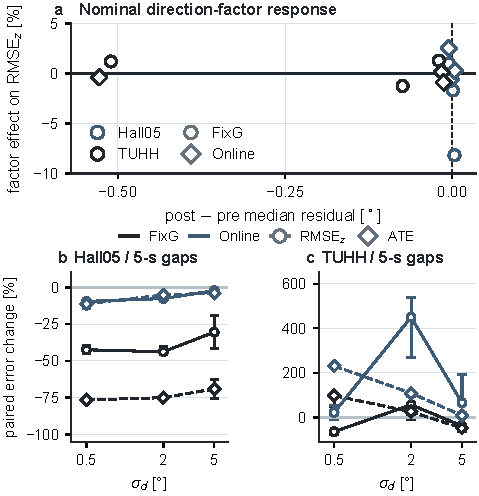
\includegraphics[width=\columnwidth]{figs/fig_direction.pdf}
\caption{Direction-factor response. \textbf{a}, Nominal residual-norm
(degree-equivalent) and RMSE$_z$ changes; color denotes trajectory, shape
denotes gravity state.
\textbf{b,c}, Dropout effects: paired medians and full ranges, with lines
connecting tested weights. Positive means worse. Failures and warnings
remain in Table~\ref{tab:direction}.}
\label{fig:direction}
\end{figure}

\subsection{Direction-Factor Response}
Nominally, factor strength has no monotonic dose response
(Fig.~\ref{fig:direction}; Table~\ref{tab:direction}). With fixed gravity, the
tightest factor worsens RMSE$_z$ by \DirStrongFGZRange{}, whereas the
intermediate factor changes RMSE$_z$/ATE by
\DirMidFGZRange{}/\DirMidFGATERange{}. Online-gravity ATE stays within
\DirGEATERange{}. Across these configurations, smaller direction residuals do not
predict smaller trajectory errors.

Under repeated 5-s gaps, the two trajectories respond differently. On Hall05, all
\NumHallDirBeneficialCells{} state--weight medians improve both errors, but the
FixG/$5^\circ$ configuration yields only $2/3$ accuracy runs because one planned run
resets; that failure is counted and was not replaced. TUHH contains both sign
reversal and metric disagreement. With FixG/$0.5^\circ$, RMSE$_z$ changes by
\TuhhDirFGStrongZ{} while ATE changes by \TuhhDirFGStrongATE{}. With online
gravity/$2^\circ$, both deteriorate by \TuhhDirGEZTwo{}/\TuhhDirGEATETwo{}.
The \NumTuhhDirArcWarnings{} complete TUHH trajectories outside the estimator
arc diagnostic band retain their metrics and carry ``A'' warnings; neither was
replaced. Thus a lower vertical error can conceal worse 3D pose, and a direction
factor can worsen both metrics. Neither increasing factor strength nor keeping
gravity online ensures an improvement.

\subsection{Accelerometer Bias and Gravity--Bias Coupling}
Accelerometer bias does not inherit gravity's removal result. \methodB{} and
\methodGB{} have median RMSE$_z$ changes of \BAMedianZ{} and
\BothMedianZ{}, with larger sequence-level ranges than \methodG{}
(Table~\ref{tab:nominal}). True-manifold interaction is \InteractionZ{}
($p=$\InteractionPZ{}) for RMSE$_z$ and \InteractionATE{}
($p=$\InteractionPATE{}) for ATE, providing no evidence of superadditivity.
The correction-nulling proxy biases the fixed-$\mathbf b_a$
comparison by \ProxyBAZ{}, confirming that it is not true removal.

The paired intervention shifts $\mathbf b_a$ by \CoupledStateInitialBA{} while
preserving $\mathbf g-\mathbf R\mathbf b_a$ within
\CoupledStateInitialHMax{}. In the handheld final 10\,s, gravity/bias remain
\CoupledHhsGRange{}/\CoupledHhsBARange{} apart, but the effective term/position
differ by only \CoupledHhsHRange{}/\CoupledHhsPoseRange{}; the vehicle estimates
return close to baseline. Handheld poses thus remain similar despite distinct
gravity and bias estimates.

\subsection{IMU Weight and Initialization}
IMU weighting does not reveal a uniform advantage for either gravity choice.
On vehicle NTU Day10, \methodG{} changes RMSE$_z$ by
\ImuDayZMin{} to \ImuDayZMax{} and ATE by \ImuDayATEMin{} to
\ImuDayATEMax{}. On vehicle NTU Night04, RMSE$_z$ changes by
\ImuNightZMin{} to \ImuNightZMax{}, but ATE worsens by
\ImuNightATEMin{} to \ImuNightATEMax{}. Maximum roll/pitch change is
\ImuStressAttMax{}.

The initialization-direction stress test also shows no monotonic FixG penalty.
Across \NumInitStressRuns{} paired runs at \InitStressAngles{}, RMSE$_z$/ATE
changes span \InitErrZMin{} to \InitErrZMax{}/\InitErrATEMin{} to
\InitErrATEMax{}, and the maximum roll/pitch change is \InitErrAttMax{}.

Across \NumDynamicFactorialPhases{} start phases and
\NumDynamicFactorialRuns{} trajectories, the dynamic-start $2\times2$ yields
no universal gravity choice. At one
stronger vehicle phase, Online and FixG produce
\FastDynamicRescueOnlineATE{} and \FastDynamicRescueFixGATE{} ATE,
respectively, while RMSE$_z$ reverses
(\FastDynamicRescueOnlineZ{} versus \FastDynamicRescueFixGZ{}). Fixed bias is
more sensitive to startup phase: both fixed-bias configurations diverge at one
low-rate handheld start. FixBa also worsens ATE in all
\NumStrongFixBaATEWorse{} stronger-motion phases (\StrongFixBaATERange{}),
although it helps at other low-rate phases. The
\NumDynamicFixedBaFailureOutcomes{} complete, finite failure outcomes are
retained rather than rerun. The phase- and metric-dependent signs do not yield
a uniform vertical Online gain.
